\documentclass[border=5mm]{standalone}
\usepackage{tikz}
\usetikzlibrary{positioning, calc, fit, arrows, decorations.pathreplacing}

\begin{document}
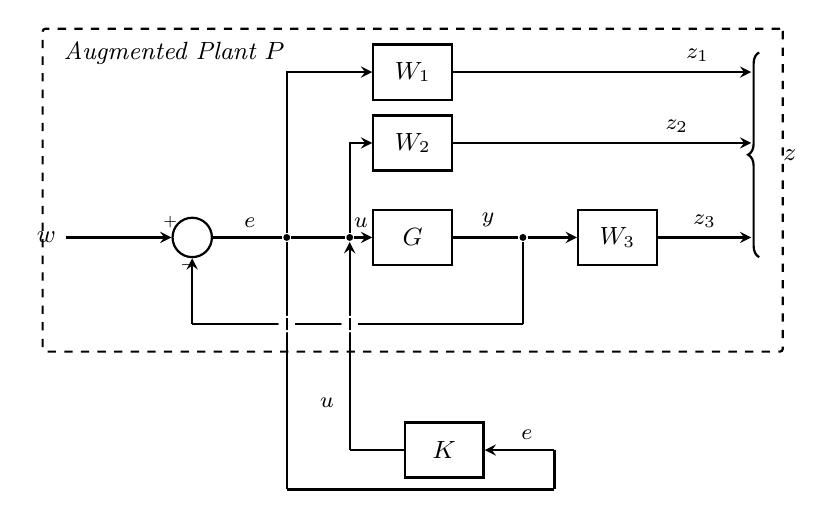
\begin{tikzpicture}[
    block/.style={draw, thick, rectangle, minimum width=10mm, minimum height=7mm,
                  font=\small},
    sum/.style={draw, thick, circle, minimum size=5mm, inner sep=0pt},
    dot/.style={fill=black, circle, inner sep=0pt, minimum size=2.5pt},
    >=stealth, thick,
]

% =================================================================
%  MAIN PATH  (y = 0)
% =================================================================
\coordinate (win) at (0, 0);
\node[sum]   (sum) at (1.6, 0)  {};
\node[block] (G)   at (4.4, 0)  {$G$};
\node[dot]   (ej)  at (2.8, 0)  {};
\node[dot]   (uj)  at (3.6, 0)  {};
\node[dot]   (yj)  at (5.8, 0)  {};

\node[font=\tiny] at ($(sum)+(145:0.34)$) {$+$};
\node[font=\tiny] at ($(sum)+(-100:0.36)$) {$-$};

\draw[->] (win) -- (sum) node[pos=0, left, font=\small] {$w$};
\draw[-]  (sum.east) -- (ej);
\draw[-]  (ej) -- (uj);
\draw[->] (uj) -- (G.west);
\draw[-]  (G.east) -- (yj);

\node[above, font=\footnotesize] at ($(sum.east)!0.5!(ej)$) {$e$};
\node[above, font=\footnotesize] at ($(uj)!0.5!(G.west)$)   {$u$};
\node[above, font=\footnotesize] at ($(G.east)!0.5!(yj)$)   {$y$};

% =================================================================
%  WEIGHTING FILTERS
% =================================================================
\node[block] (W1) at (4.4, 2.1)  {$W_1$};
\node[block] (W2) at (4.4, 1.2)  {$W_2$};
\node[block] (W3) at (7.0, 0)    {$W_3$};

\draw[->] (ej) |- (W1.west);
\draw[->] (uj) |- (W2.west);
\draw[->] (yj) -- (W3.west);

\pgfmathsetmacro{\zx}{8.7}
\draw[->] (W1.east) -- (\zx, 2.1) node[pos=0.82, above, font=\footnotesize] {$z_1$};
\draw[->] (W2.east) -- (\zx, 1.2) node[pos=0.75, above, font=\footnotesize] {$z_2$};
\draw[->] (W3.east) -- (\zx, 0)   node[pos=0.50, above, font=\footnotesize] {$z_3$};

\draw[decorate, decoration={brace, amplitude=4pt, mirror}]
    (\zx+0.1, 2.35) -- (\zx+0.1, -0.25)
    node[midway, right=5pt, font=\small] {$z$};

% =================================================================
%  y-FEEDBACK inside P
% =================================================================
\draw[-]  (yj) -- (5.8, -1.1);
\draw[-]  (5.8, -1.1) -- (1.6, -1.1);
\draw[->] (1.6, -1.1) -- (sum.south);

% =================================================================
%  DASHED BOX: Augmented Plant P
% =================================================================
\node[draw, dashed, thick, rounded corners=1pt,
      inner sep=0pt,
      fit={(-0.3, 2.65) (9.1, -1.45)}]
      (Pbox) {};
\node[anchor=north west, font=\itshape\small]
      at ($(Pbox.north west)+(0.15,-0.05)$)
      {Augmented Plant $P$};

% =================================================================
%  CONTROLLER K
% =================================================================
\node[block] (K) at (4.8, -2.7) {$K$};

% u: K.west -> left -> up to uj
\draw[-]  (K.west) -- (3.6, -2.7);
\draw[->] (3.6, -2.7) -- (uj);
\node[left=2pt, font=\footnotesize] at (3.6, -2.1) {$u$};

% e: ej -> down -> right under K -> up -> left into K.east
\draw[-] (ej) -- (2.8, -3.2);
\draw[-] (2.8, -3.2) -- (6.2, -3.2);
\draw[-] (6.2, -3.2) -- (6.2, -2.7);
\draw[->] (6.2, -2.7) -- (K.east);
\node[above, font=\footnotesize] at (5.85, -2.7) {$e$};

% =================================================================
%  Wire-crossing bridges
% =================================================================
% u crosses y-feedback at (3.6, -1.1)
\fill[white] (3.6, -1.1) circle (3pt);
\draw[-] (3.6, -1.18) -- (3.6, -1.02);

% e crosses y-feedback at (2.8, -1.1)
\fill[white] (2.8, -1.1) circle (3pt);
\draw[-] (2.8, -1.18) -- (2.8, -1.02);

\end{tikzpicture}
\end{document}
